\documentclass{article}
\usepackage[utf8]{inputenc}
\usepackage{packages}
\usepackage{siunitx}

\title{Amplificatore differenziale}
\date{Luglio 2020}
\author{Elena Acinapura}

\begin{document}

\maketitle

Valori dei componenti usati per alcune stime
\begin{itemize}
    \item ${R_C} = 9.830\pm0.001~\si{\kilo\ohm}$ 
    \item ${R_E} = 119.25\pm0.03~\si{\ohm}$
    \item $R_1 = 9.924\pm1~\si{\kilo\ohm}$
\end{itemize}


\section*{Configurazione con resistenza}
\begin{figure}[h!]
    \centering
    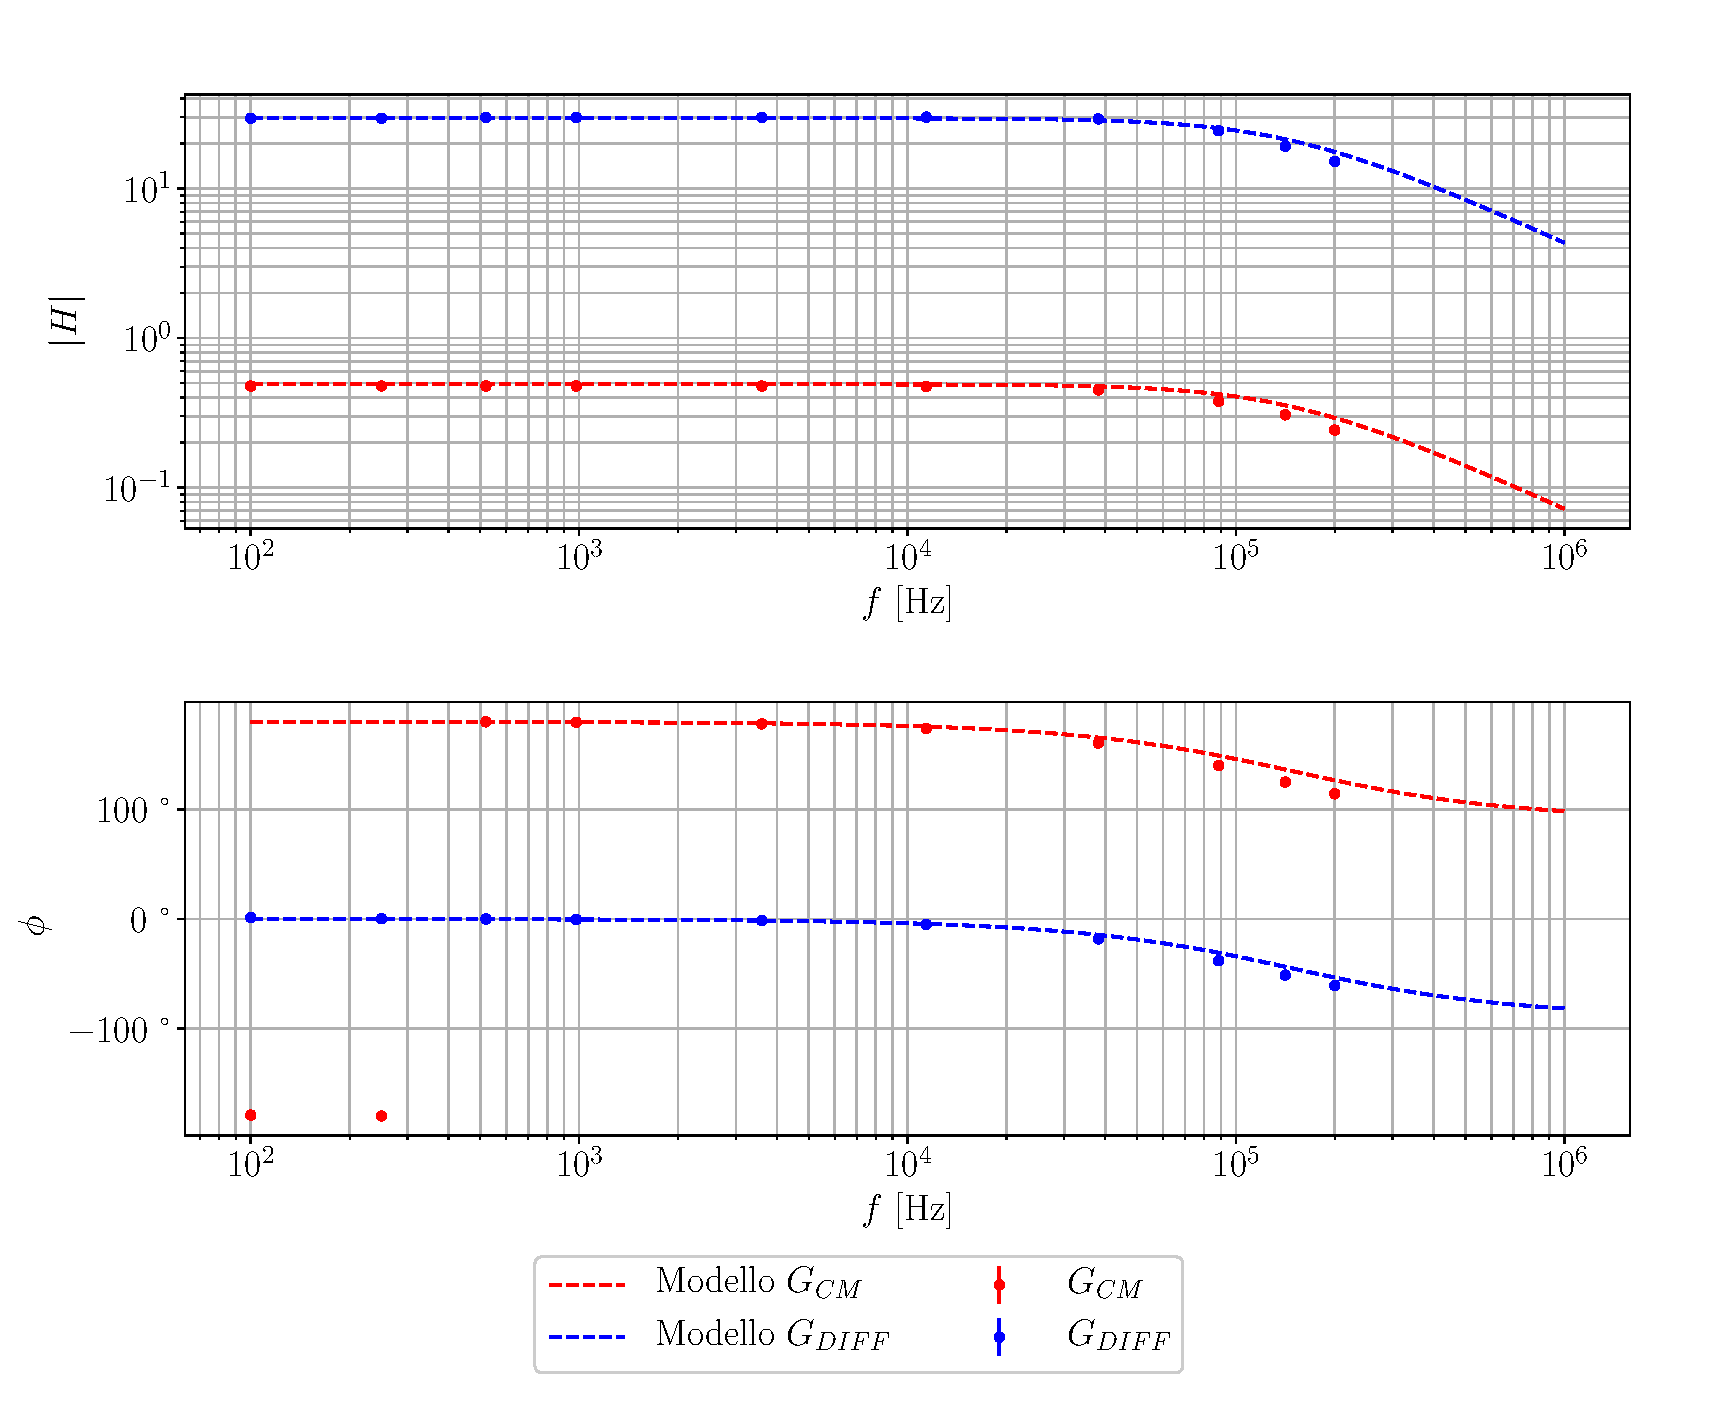
\includegraphics[scale = 0.6]{Grafici/resistenza.eps}
    \caption{Funzione di trasferimento.}
    \label{fig:resistenza}
\end{figure}
Il moodello teorico è ottenuto aggiungendo un carico di impedenza $Z_{OSC}$ in uscita dal circuito, composto da un parallelo di $$R_{OSC} = 1~\si{\mega\ohm} \quad \text{e} \quad C_{OSC} = 110~\si{\pico\farad}$$
Si è usato il circuito equivalente di Thevenin, usando come $V_{eq}$ il valore di guadagno medio a basse frequenze (prime 5 frequenze) e come resistenza in uscita $$R_{out} = R_C$$

\subsection*{Stime di parametri incogniti}
$r_e$ e CMRR ottenuti per media su sulle prime 5 frequenze basse:
$$ r_e = 45\pm 1~\si{\ohm}$$
$$ CMRR = 63\pm 1$$
Una possibile stima teorica per $r_e$ se nel transistor passa una corrente quiescente di $0.7~\si{\milli\ampere}$ è di $\simeq 35.7~\si{\ohm}$.

\section*{Configurazione con sorgente BJT}
\begin{figure}[h!]
    \centering
    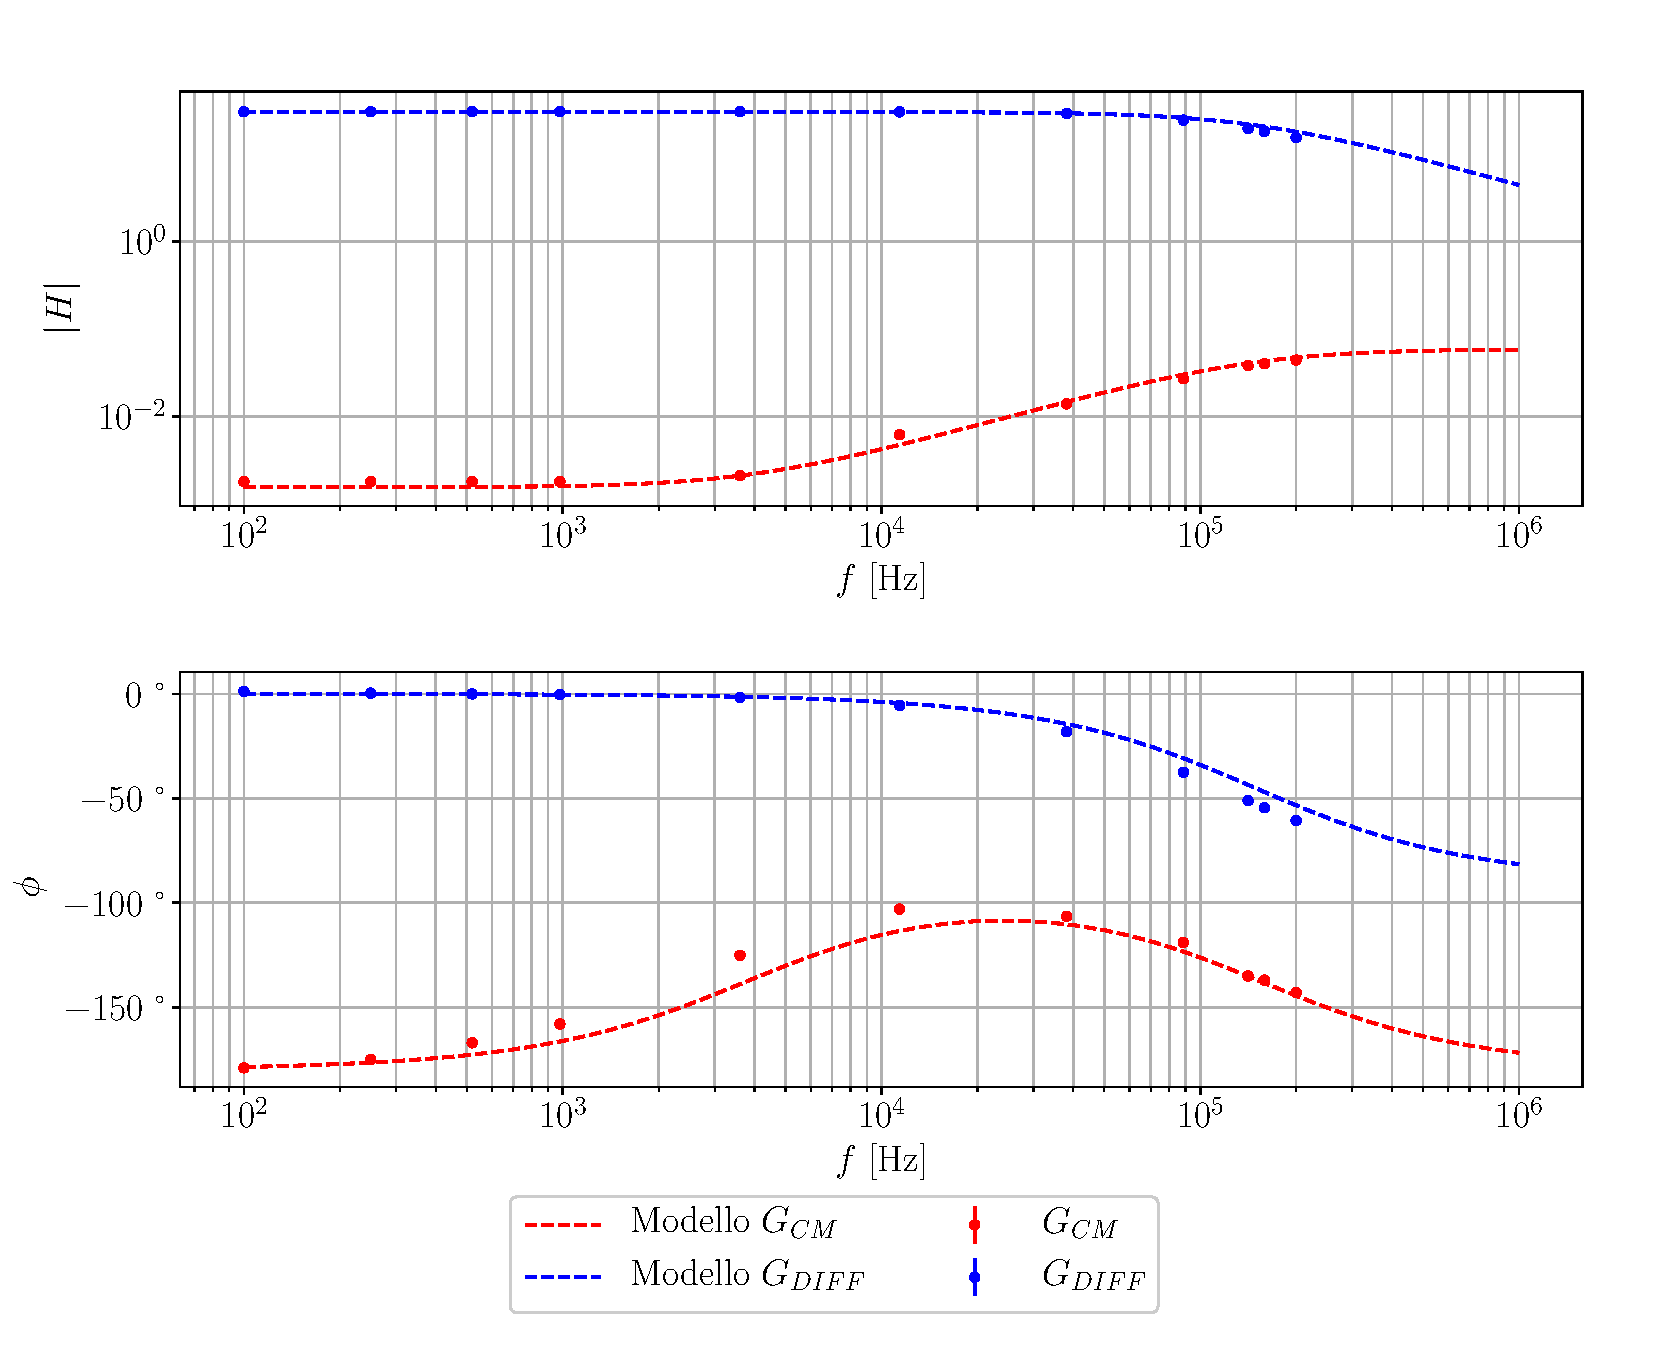
\includegraphics[scale = 0.6]{Grafici/sorgente.eps}
    \caption{Funzione di trasferimento}
    \label{fig:resistenza}
\end{figure}
Il modello teorico per il guadagno differenziale è ottenuto come nella configurazione senza sorgente, mentre per il guadagno modo comune si è utilizzata, per stimare $V_{eq}$, la stima di $Z_s$, spiegata sotto. $R_{out}$ è rimasta sempre $R_C$.

\subsection*{Stime di parametri incogniti}
$r_e$ e CMRR ottenuti per media su sulle prime 5 frequenze basse:
$$ r_e = 43.2\pm 0.2~\si{\ohm}$$
$$ CMRR = (16\pm7)\cdot 10^{3}$$
Stimo $Z_s$ dalla relazione $$G_{CM} = \frac{R_C}{2 Z_s}$$
Scrivo $Z_s$ come un parallelo di $R_s$ e $C_s$, stimo $R_s$ da una media sulle 4 frequenze più basse e $C_s$ da una media sulle 5 frequenze più alte.
$$ R_s = 3.1\pm0.5~\si{\mega\ohm}$$
$$C_s = 13\pm7~\si{\pico\farad}$$

\section*{Valutazione incertezze}
Per i guadagni modo comune con resistenza, differenziale con resistenza e differenziale con sorgente è stata presa una solo acquisizione temporale per frequenza. In quel caso:
\begin{itemize}
    \item si sono calcolate le ampiezze complesse $C$ per il segnale in entrata e in uscita con un fit sinusoidale
    \item si è stimata l'incertezza su $\abs{C}$ come il $3\%$ della scala verticale dell'oscilloscopio (full scale)
    \item si è stimata l'incertezza su $\arg{C}$ come incertezza $2\pi f \Delta t$, con $\Delta t$ pari a $8\cdot 10^{-4}$ per la full scale sui tempi dell'oscilloscopio
\end{itemize}
Per il guadagno modo comune con sorgente sono state acquisite 5 serie temporali per frequenza e l'incertezza sulla funzione di trasferimento è stata scelta come la deviazione standard dei valori su misure ripetute.

\end{document}

